\chapter{Manual de usuario}

Pese a que se ha priorizado la usabilidad de la aplicación durante su desarrollo, en este apartado se especificarán los pasos a seguir para utilizar las funcionalidades que ofrece, ayudándonos de capturas cuando sea necesario. La parte más importante de este manual de usuario es la sección dedicada a mostrar los botones del mando que se pueden usar en cada escena del juego y las funcionalidades que ofrecen.

\section{Instalación/Ejecución de la aplicación}

Pese a que se trate este aspecto de una forma completa en el apartado \ref{sec:ejecucion} del manual técnico, a nivel de usuario la forma ideal de comenzar la ejecución del programa es simplemente utilizar la interfaz del sistema de archivos de macOS y hacer doble \textit{click} sobre el ejecutable llamado \textbf{\textit{It\_Fights.app}}. No hay pasos relacionados con la instalación en si misma sino que simplemente se debe de estar en posesión del ejecutable.


\section{Controles de la aplicación}
\label{sec:controles}
Desde el punto de vista de un usuario común, la aplicación prioriza el uso único del mando. Para explicar el funcionamiento de cada uno de los botones (o los equivalentes en mandos de otras marcas) se hará uso de la figura \ref{controles:mando}\footnote{Imagen oficial de la documentación de Microsoft extraída de: \\ \url{https://support.xbox.com/es-ES/xbox-360/accessories/controllers}}.

\begin{figure}
	\centerline{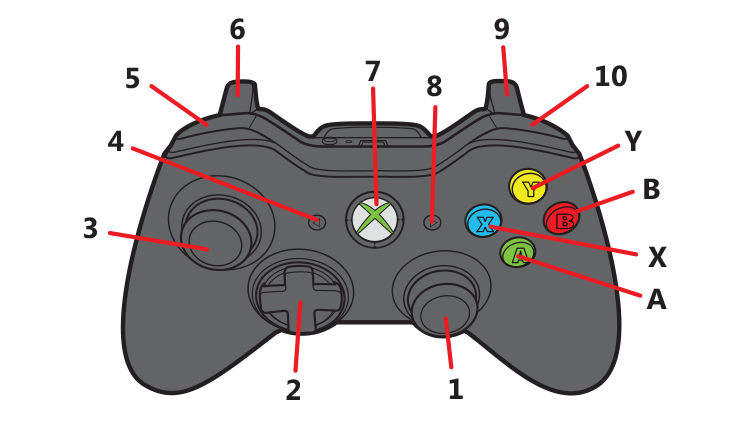
\includegraphics[width=12cm]{otros/graphicalInterface/mando.png}}
	\caption{Mando de Xbox360}
	\label{controles:mando}
\end{figure}

\subsection{Controles del menú}

Los controles de la escena del menú a la hora de usar el mando son los siguientes:

\begin{itemize}
	\item \textbf{\textit{D-Pad}}: Identificado con el número \textbf{2} en la figura \ref{controles:mando}. Usado para mover arriba y abajo las opciones seleccionadas del menú, mover el D-PAD a izquierda y derecha no tendrá efecto.
	\item \textbf{\textit{Botón X}} Identificado con la letra \textbf{X} en la figura \ref{controles:mando}. Usado para ejecutar la opción seleccionada actualmente.
\end{itemize}

\subsection{Controles de combate}

Los controles a la hora de controlar a uno de los jugadores (o a ambos si se dispone de dos mandos conectados en la opción de jugador contra jugador) son los siguiente:

\begin{itemize}
	\item \textbf{\textit{Joystick izquierdo}}: Identificado con el número \textbf{3} en la figura \ref{controles:mando}. Usado para mover al jugador en cualquier dirección (360 grados). Si se inclina ligeramente el movimiento del personaje será más lento permitiendo variar la velocidad del mismo.
	\item \textbf{\textit{Botón A}} Identificado con la letra \textbf{A} en la figura \ref{controles:mando}. Usado para realizar un ataque en la dirección en la que se está mirando.
	\item \textbf{\textit{Botón B}} Identificado con la letra \textbf{B} en la figura \ref{controles:mando}. Usado para realizar una acción defensiva o \textit{parry}\footnote{Término usado en esgrima para bloquear y/o reflejar un ataque inminente hacia el contrincante} en la dirección que se está mirando.
	\item \textbf{\textit{Botón Back}} Identificado con el número \textbf{4} en la figura \ref{controles:mando}. Usado para volver al menú saliendo de la pelea.
\end{itemize}

\subsection{Controles avanzados}

Además, se pueden usar las flechas del teclado para iterar sobre las opciones del menú y la tecla \textit{intro} para ejecutar la opción. Otra opción disponible es abrir y cerrar la consola de la aplicación al introducir el carácter del teclado \textbf{\textbackslash} conocido como \textbf{barra invertida}. Con la consola abierta, todos los caracteres que introduzcamos con el teclado se agregarán a la línea de entrada de la consola. Además podremos usar la tecla \textit{intro} para confirmar el comando introducido. \textbf{Importante}: Esta opción está disponible solamente para usuarios avanzados y preferentemente con conocimiento interno de la aplicación por lo que no se incluirán una lista de los mensajes permitidos.

\section{Uso de las diferentes escenas}

Utilizaremos esta sección para mostrar una vista de las escenas que se pueden dar y especificar el comportamiento de las mismas de cara al usuario o jugador.

\bigskip

Como nota adicional se mencionará aquí la posibilidad de cambiar el tamaño de la ventana de la aplicación en cualquier momento. Al hacerlo siempre se mantendrá la relación de aspecto y se escalará la imagen vista para que no se produzcan errores visuales.

\subsection{Uso del menú}

\begin{figure}[h]
	\centerline{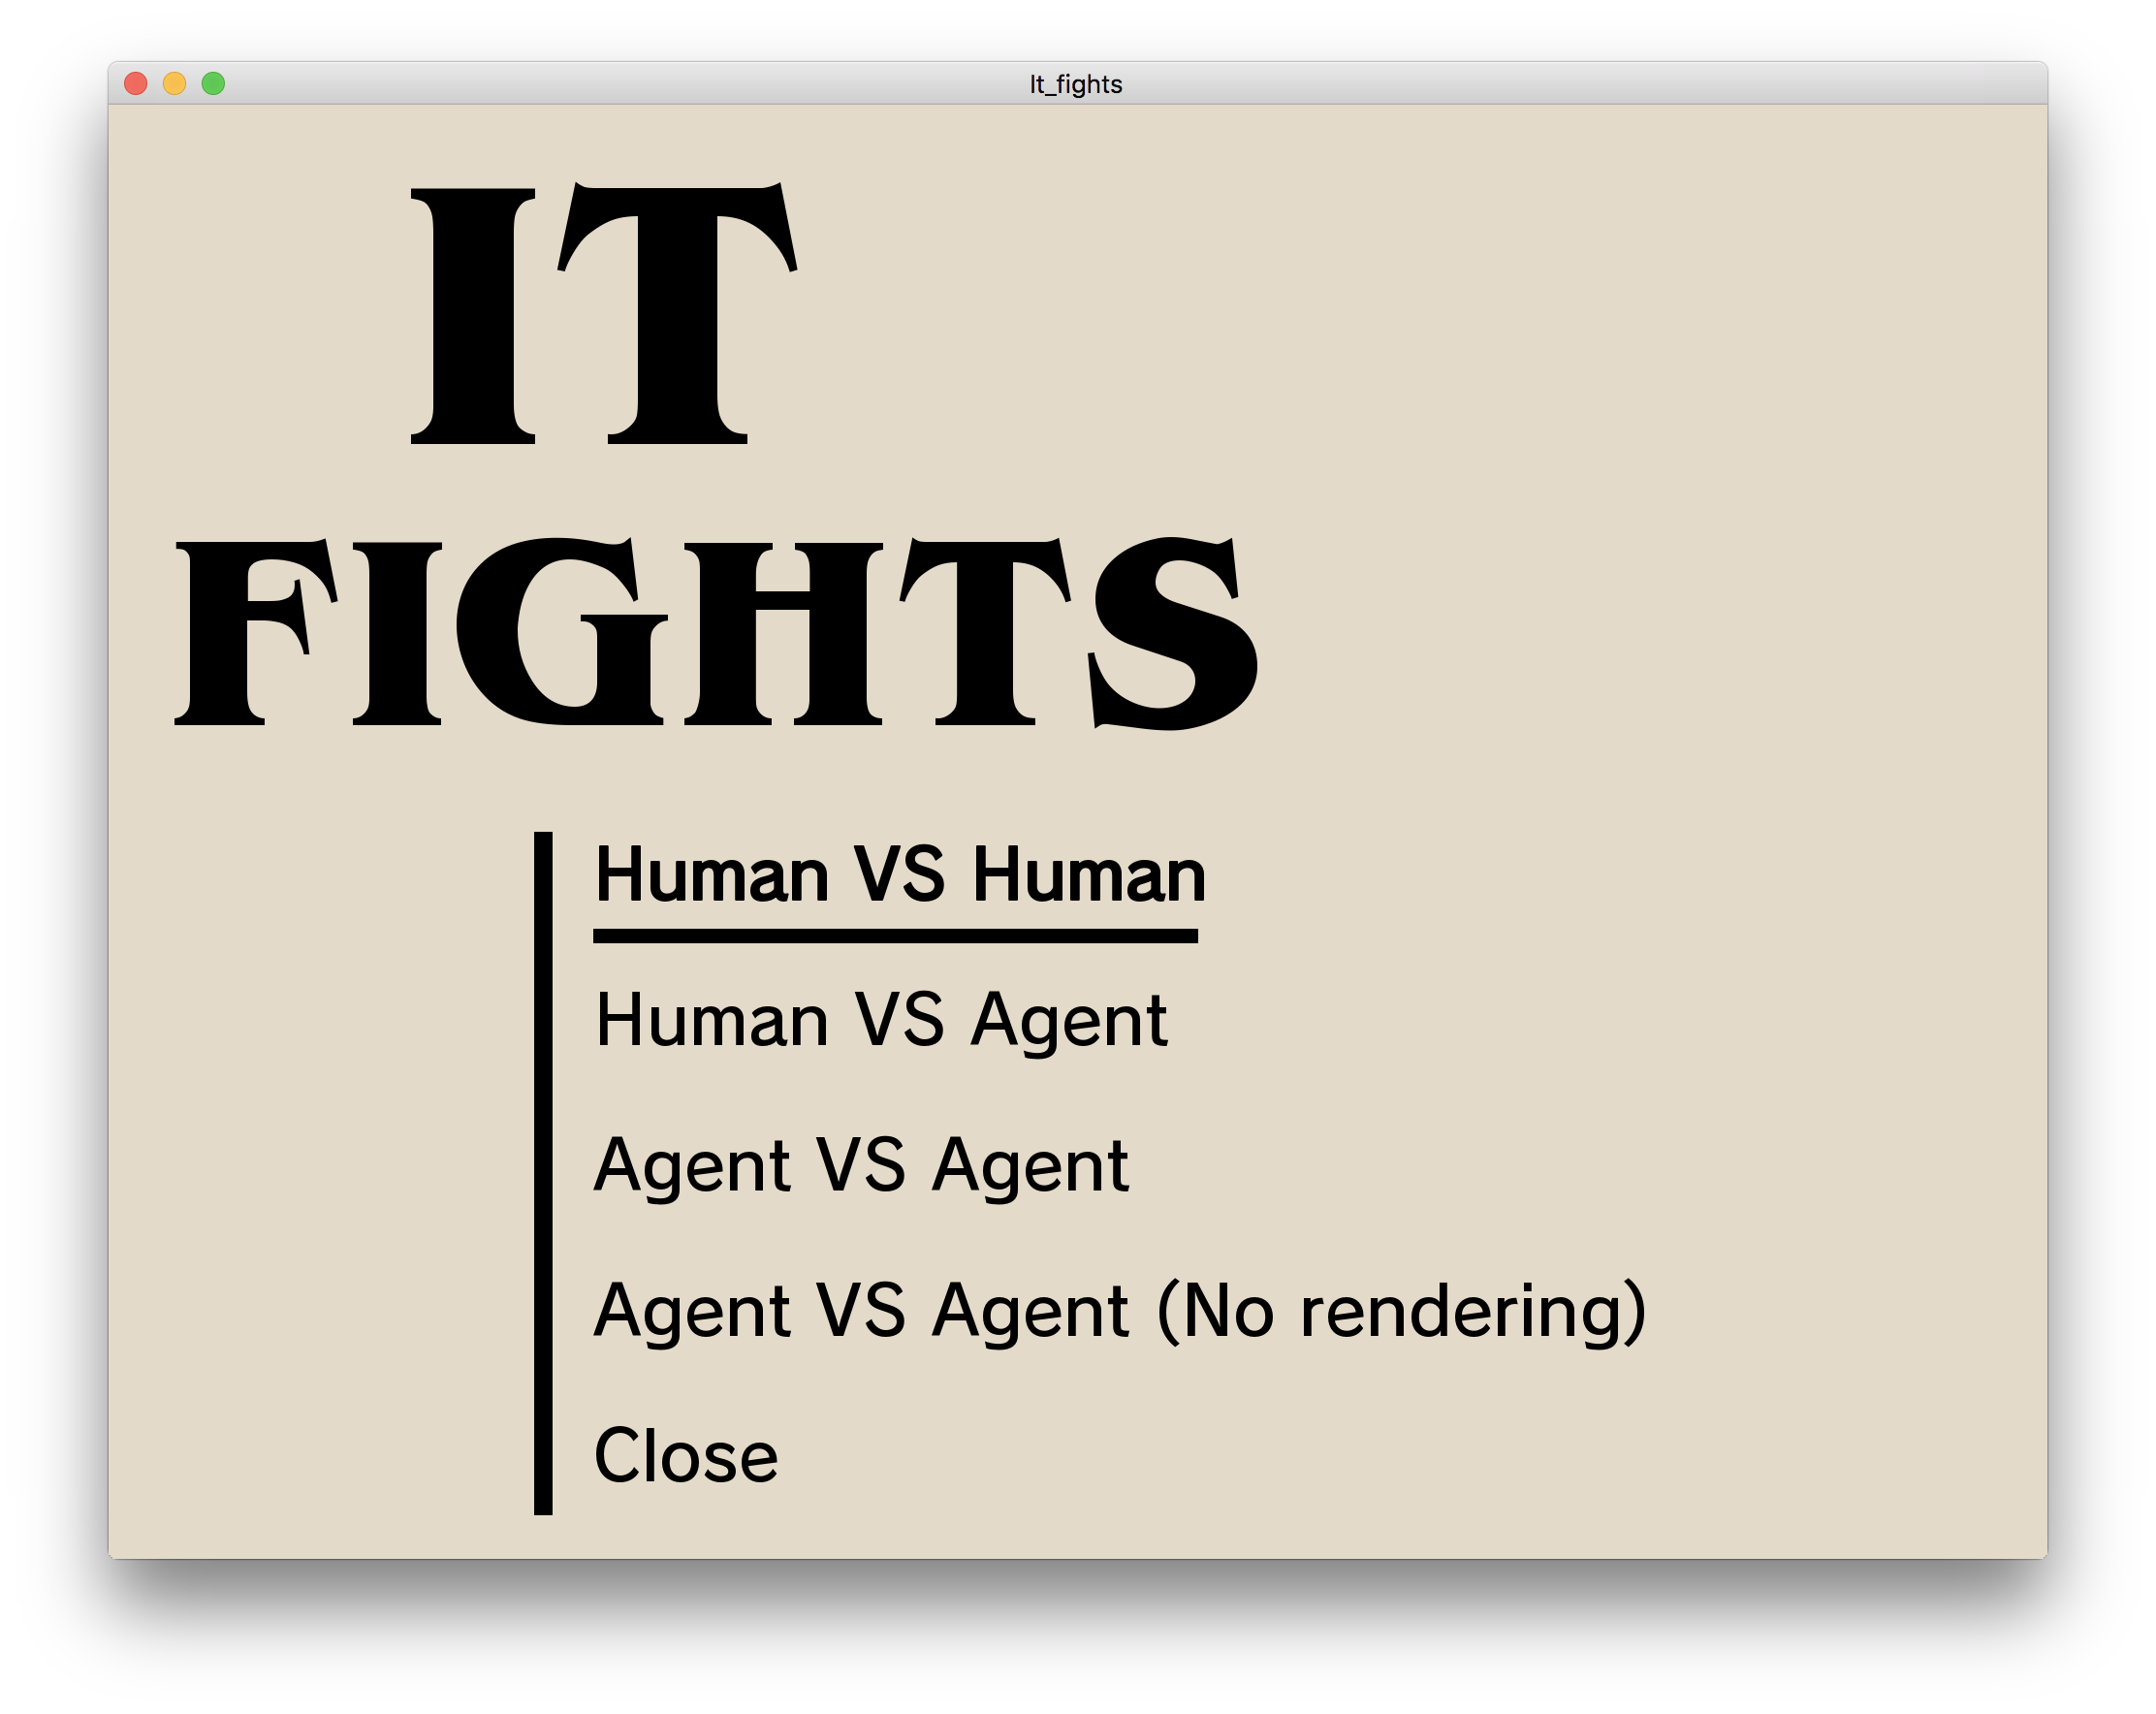
\includegraphics[width=17cm]{otros/manual/menu1.png}}
	\caption{Menú al iniciar la aplicación}
	\label{uso:menu}
\end{figure}

\begin{figure}[h]
	\centerline{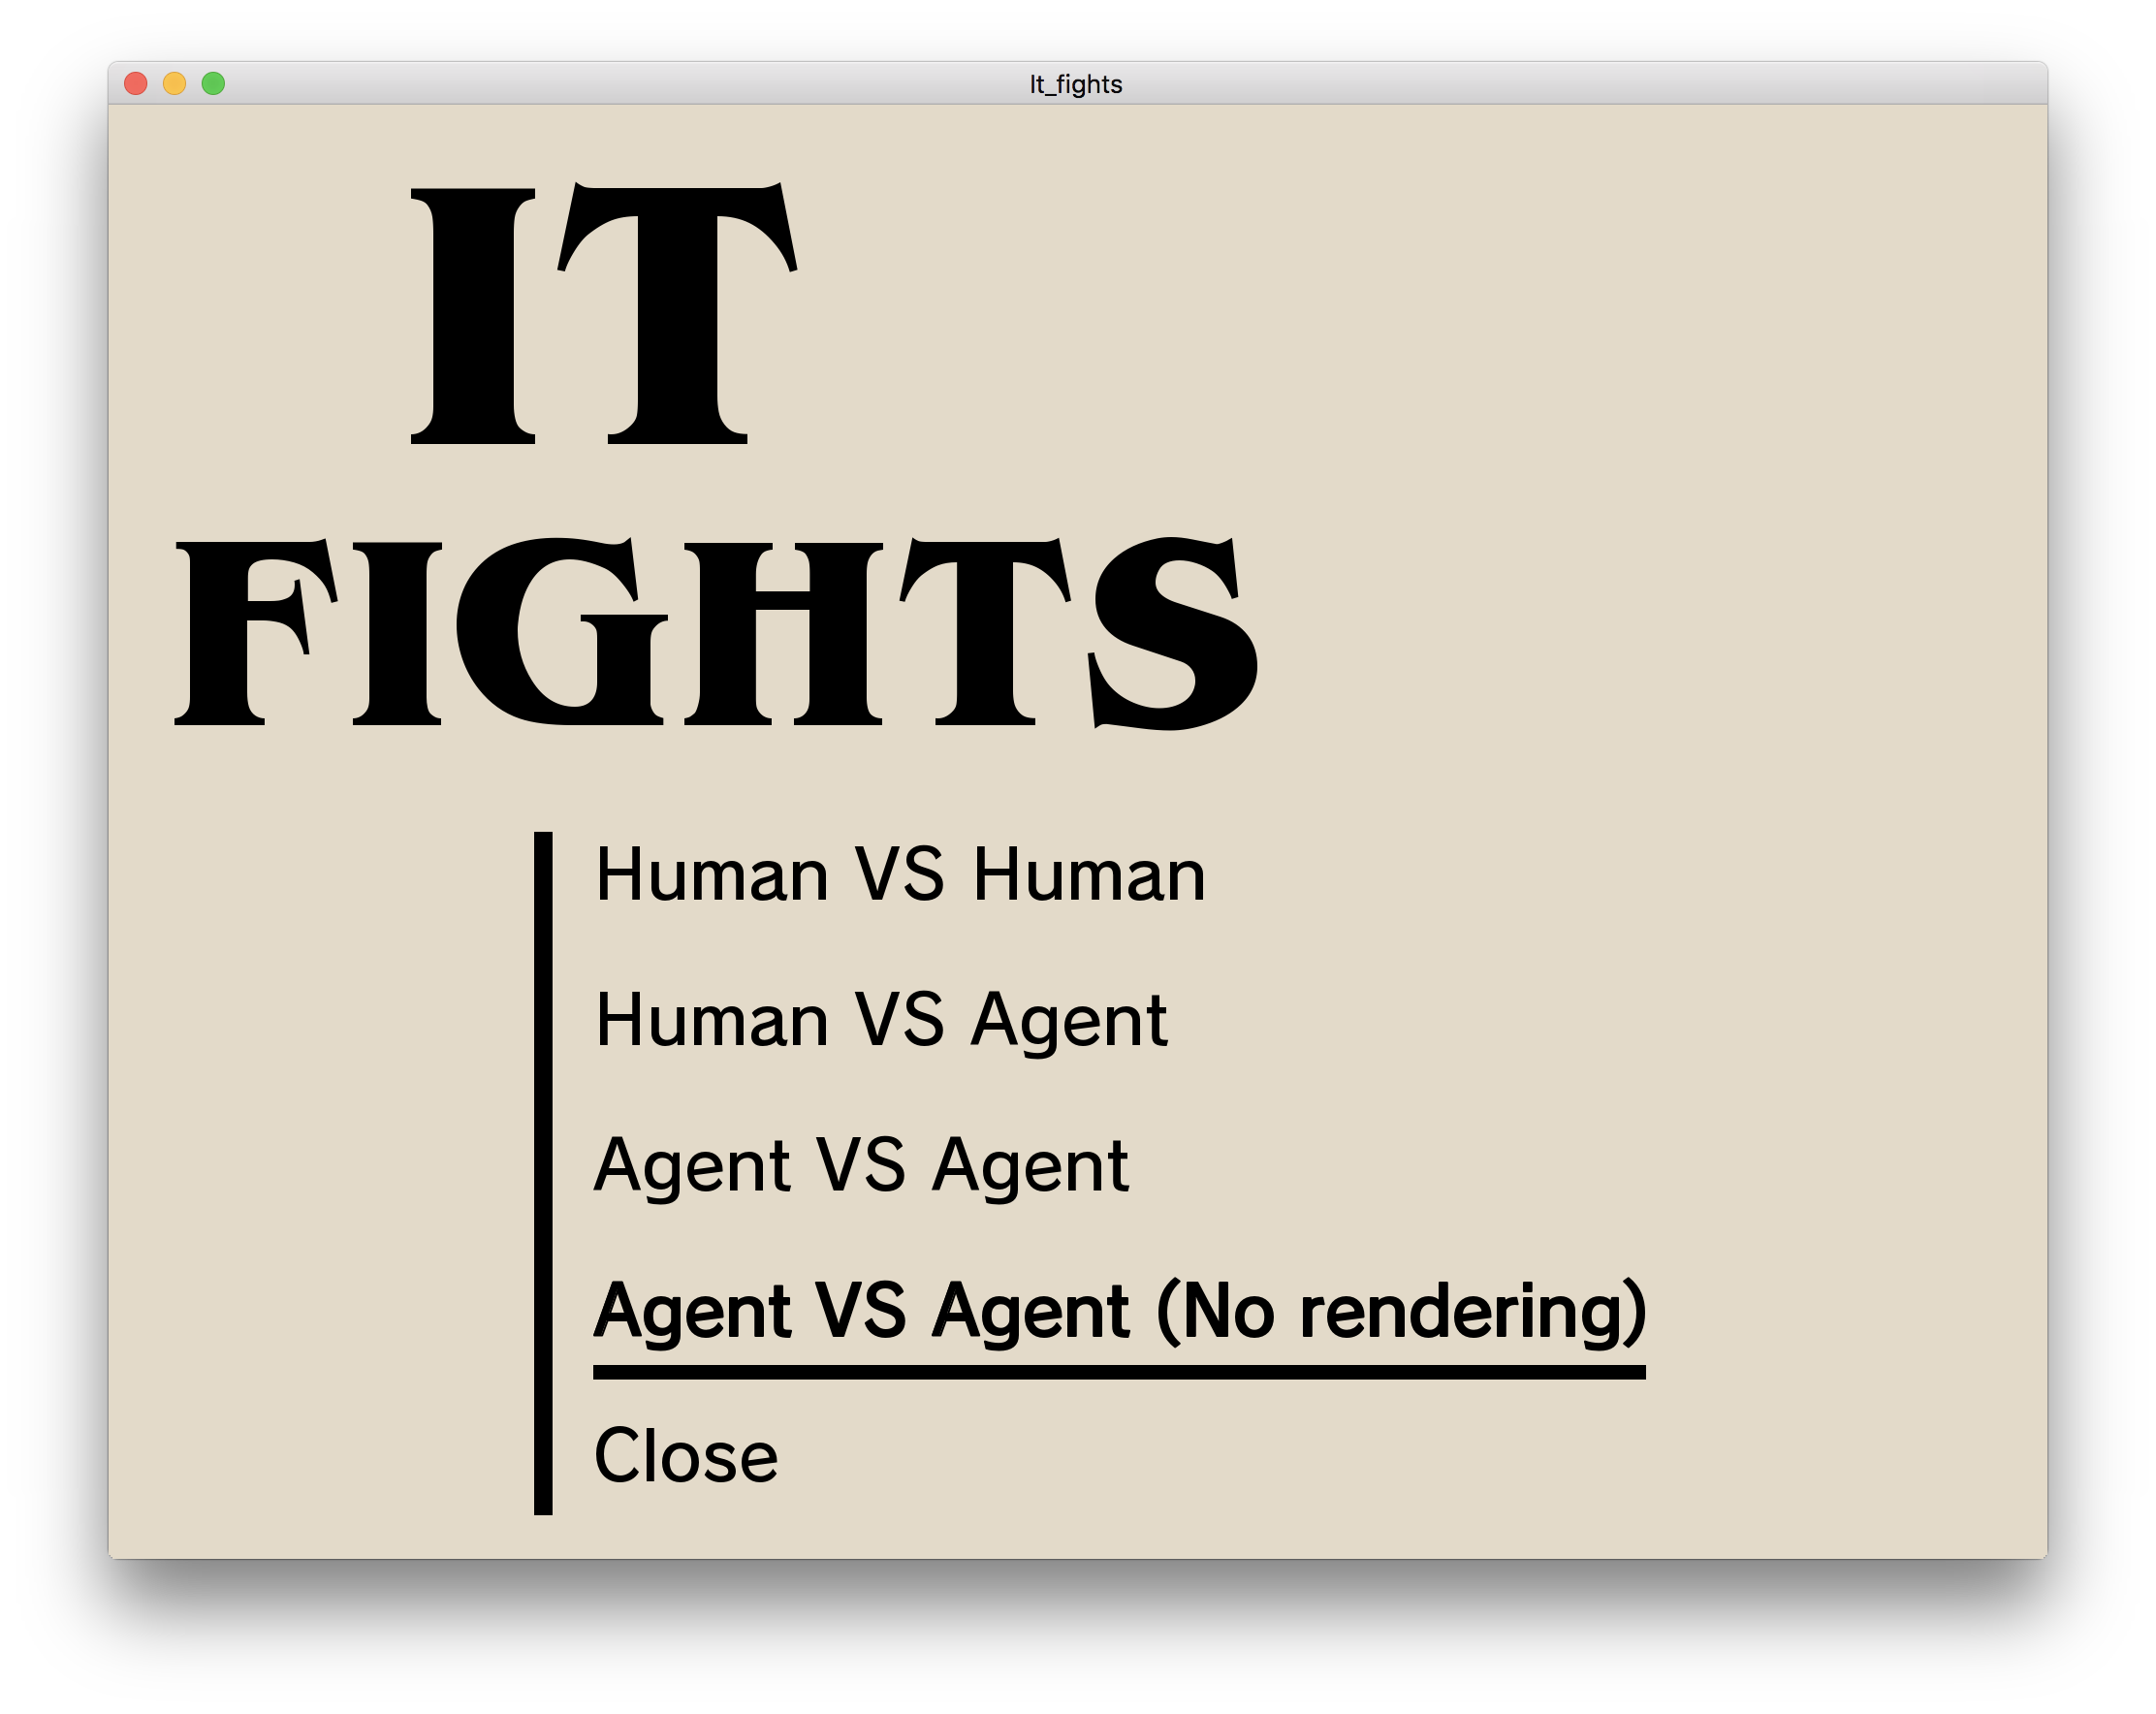
\includegraphics[width=17cm]{otros/manual/menu2.png}}
	\caption{Menú al cambiar de opción}
	\label{uso:menu2}
\end{figure}

En las figuras \ref{uso:menu} y \ref{uso:menu2} vemos el menú de la aplicación. En la primera figura (\ref{uso:menu}) se observa cómo la opción preseleccionada por defecto es la primera, si movemos con el D-PAD o el las flechas del teclado la selección o bien dos veces arriba o tres veces abajo llegaremos a la opción mostrada en la segunda figura (\ref{uso:menu}). Al cambiar de opción se moverá la barra que subraya la nueva opción seleccionada, dicha opción también se mostrará en negrita y se oirá un sonido similar a un silbido al realizar dicho cambio.

\bigskip

Al pulsar el botón de ejecutar (\textbf{X}) se ejecutará la opción seleccionada en ese momento, la ejecución de cada opción implica las siguientes acciones:

\begin{enumerate}
	\item \textbf{\textit{Human VS Human}}: Se comienza el combate entre dos jugadores (necesarios dos mandos conectados al equipo para controlar a ambos).
	\item \textbf{\textit{Human VS Agent}}: Se comienza el combate contra el agente que ha aprendido previamente.
	\item \textbf{\textit{Agent VS Agent}}: Se enfrentan dos enemigos, el basado en reglas y el agente que ha aprendido.
	\item \textbf{\textit{Agent VS Agent (No Rendering)}}: Se enfrentan los dos enemigos durante 100 simulaciones, las mismas no se mostrarán por pantalla (\textbf{Importante}: Solo con fines de demostración, para mostrar las capacidades y rendimiento del motor y del agente).
	\item \textbf{\textit{Close}}: Cierra la ventana y la aplicación.
\end{enumerate}

\subsection{Combate}

\begin{figure}[h]
	\centerline{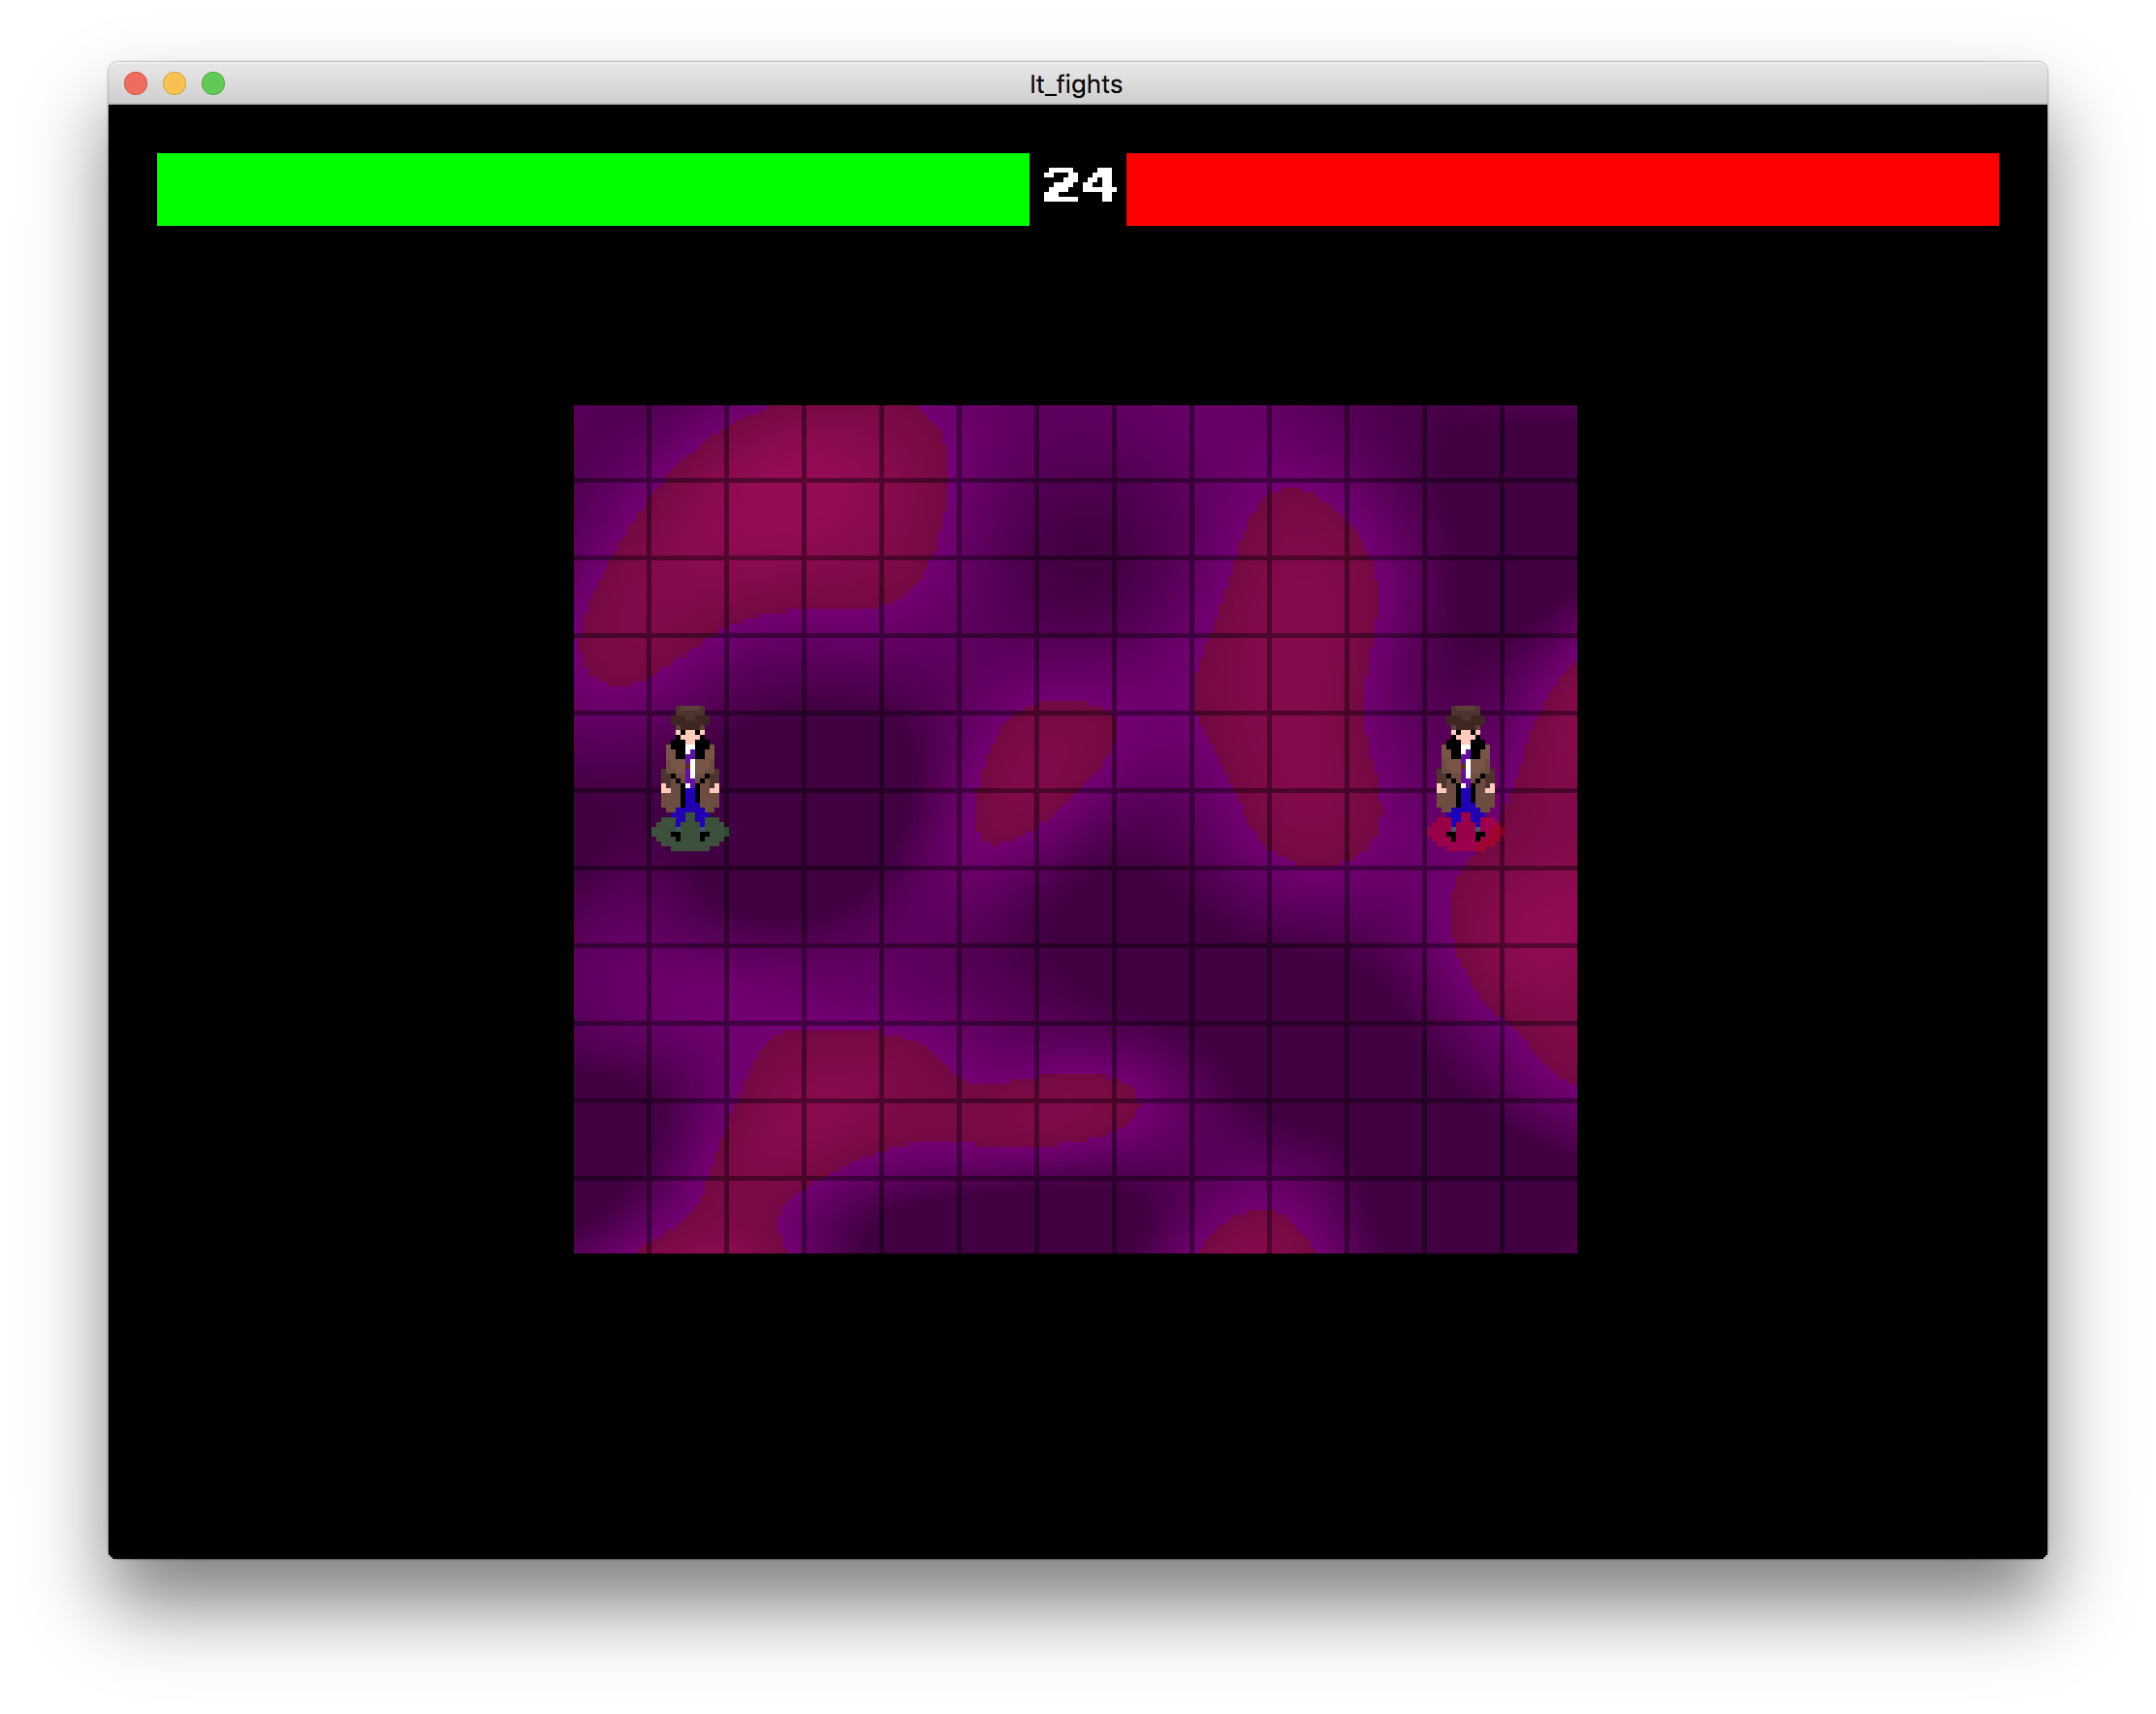
\includegraphics[width=17cm]{otros/manual/pelea1.png}}
	\caption{Inicio del combate}
	\label{uso:pelea1}
\end{figure}


\begin{figure}[h]
	\centerline{
\includegraphics[width=14cm]{otros/manual/atacando1.png}}
	\caption{Personaje atacando}
	\label{uso:ataque}
\end{figure}

\begin{figure}[h]
	\centerline{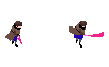
\includegraphics[width=14cm]{otros/manual/parry.png}}
	\caption{Personaje haciendo \textit{parry}}
	\label{uso:parry}
\end{figure}


Si se elige una de las dos primeras opciones se entrará en una escena de combate en la que se puede controlar al jugador, dicha escena se puede ver en la figura \ref{uso:pelea1}. Las mecánicas del combate son las siguientes:

\begin{itemize}
	\item \textbf{Moverse}: El personaje se moverá en la dirección deseada. Se puede reducir la velocidad de movimiento reduciendo el ángulo del \textit{joystick}. El personaje estará mirando siempre para la dirección en la que se está moviendo o la última en la que se ha movido si está quieto.
	\item \textbf{Atacar}: Al atacar el personaje realizará una animación en la dirección en la que se está mirando, si el enemigo está en esa dirección y a rango de ataque será dañado a menos que esté realizando un \textit{parry}. El ataque implica un pequeño desplazamiento del personaje hacia delante. Se puede ver en la figura \ref{uso:ataque}.
	\item \textbf{Defenderse o \textit{parry}}: Al realizar un \textit{parry} el personaje será invulnerable durante medio segundo. Sin embargo, si durante ese medio segundo no se para ningún ataque se entrará en un periodo de descanso durante otro medio segundo donde no se podrá mover, atacar o defenderse. Si por el contrario sí se defiende con éxito entonces se podrá realizar un ataque gratuito al personaje enemigo. Se puede ver en la figura \ref{uso:parry}.
	\item \textbf{Salir de la partida}: Se sale del combate volviendo al menú de la aplicación. 
\end{itemize}


\subsection{Consola}

\begin{figure}[h]
	\centerline{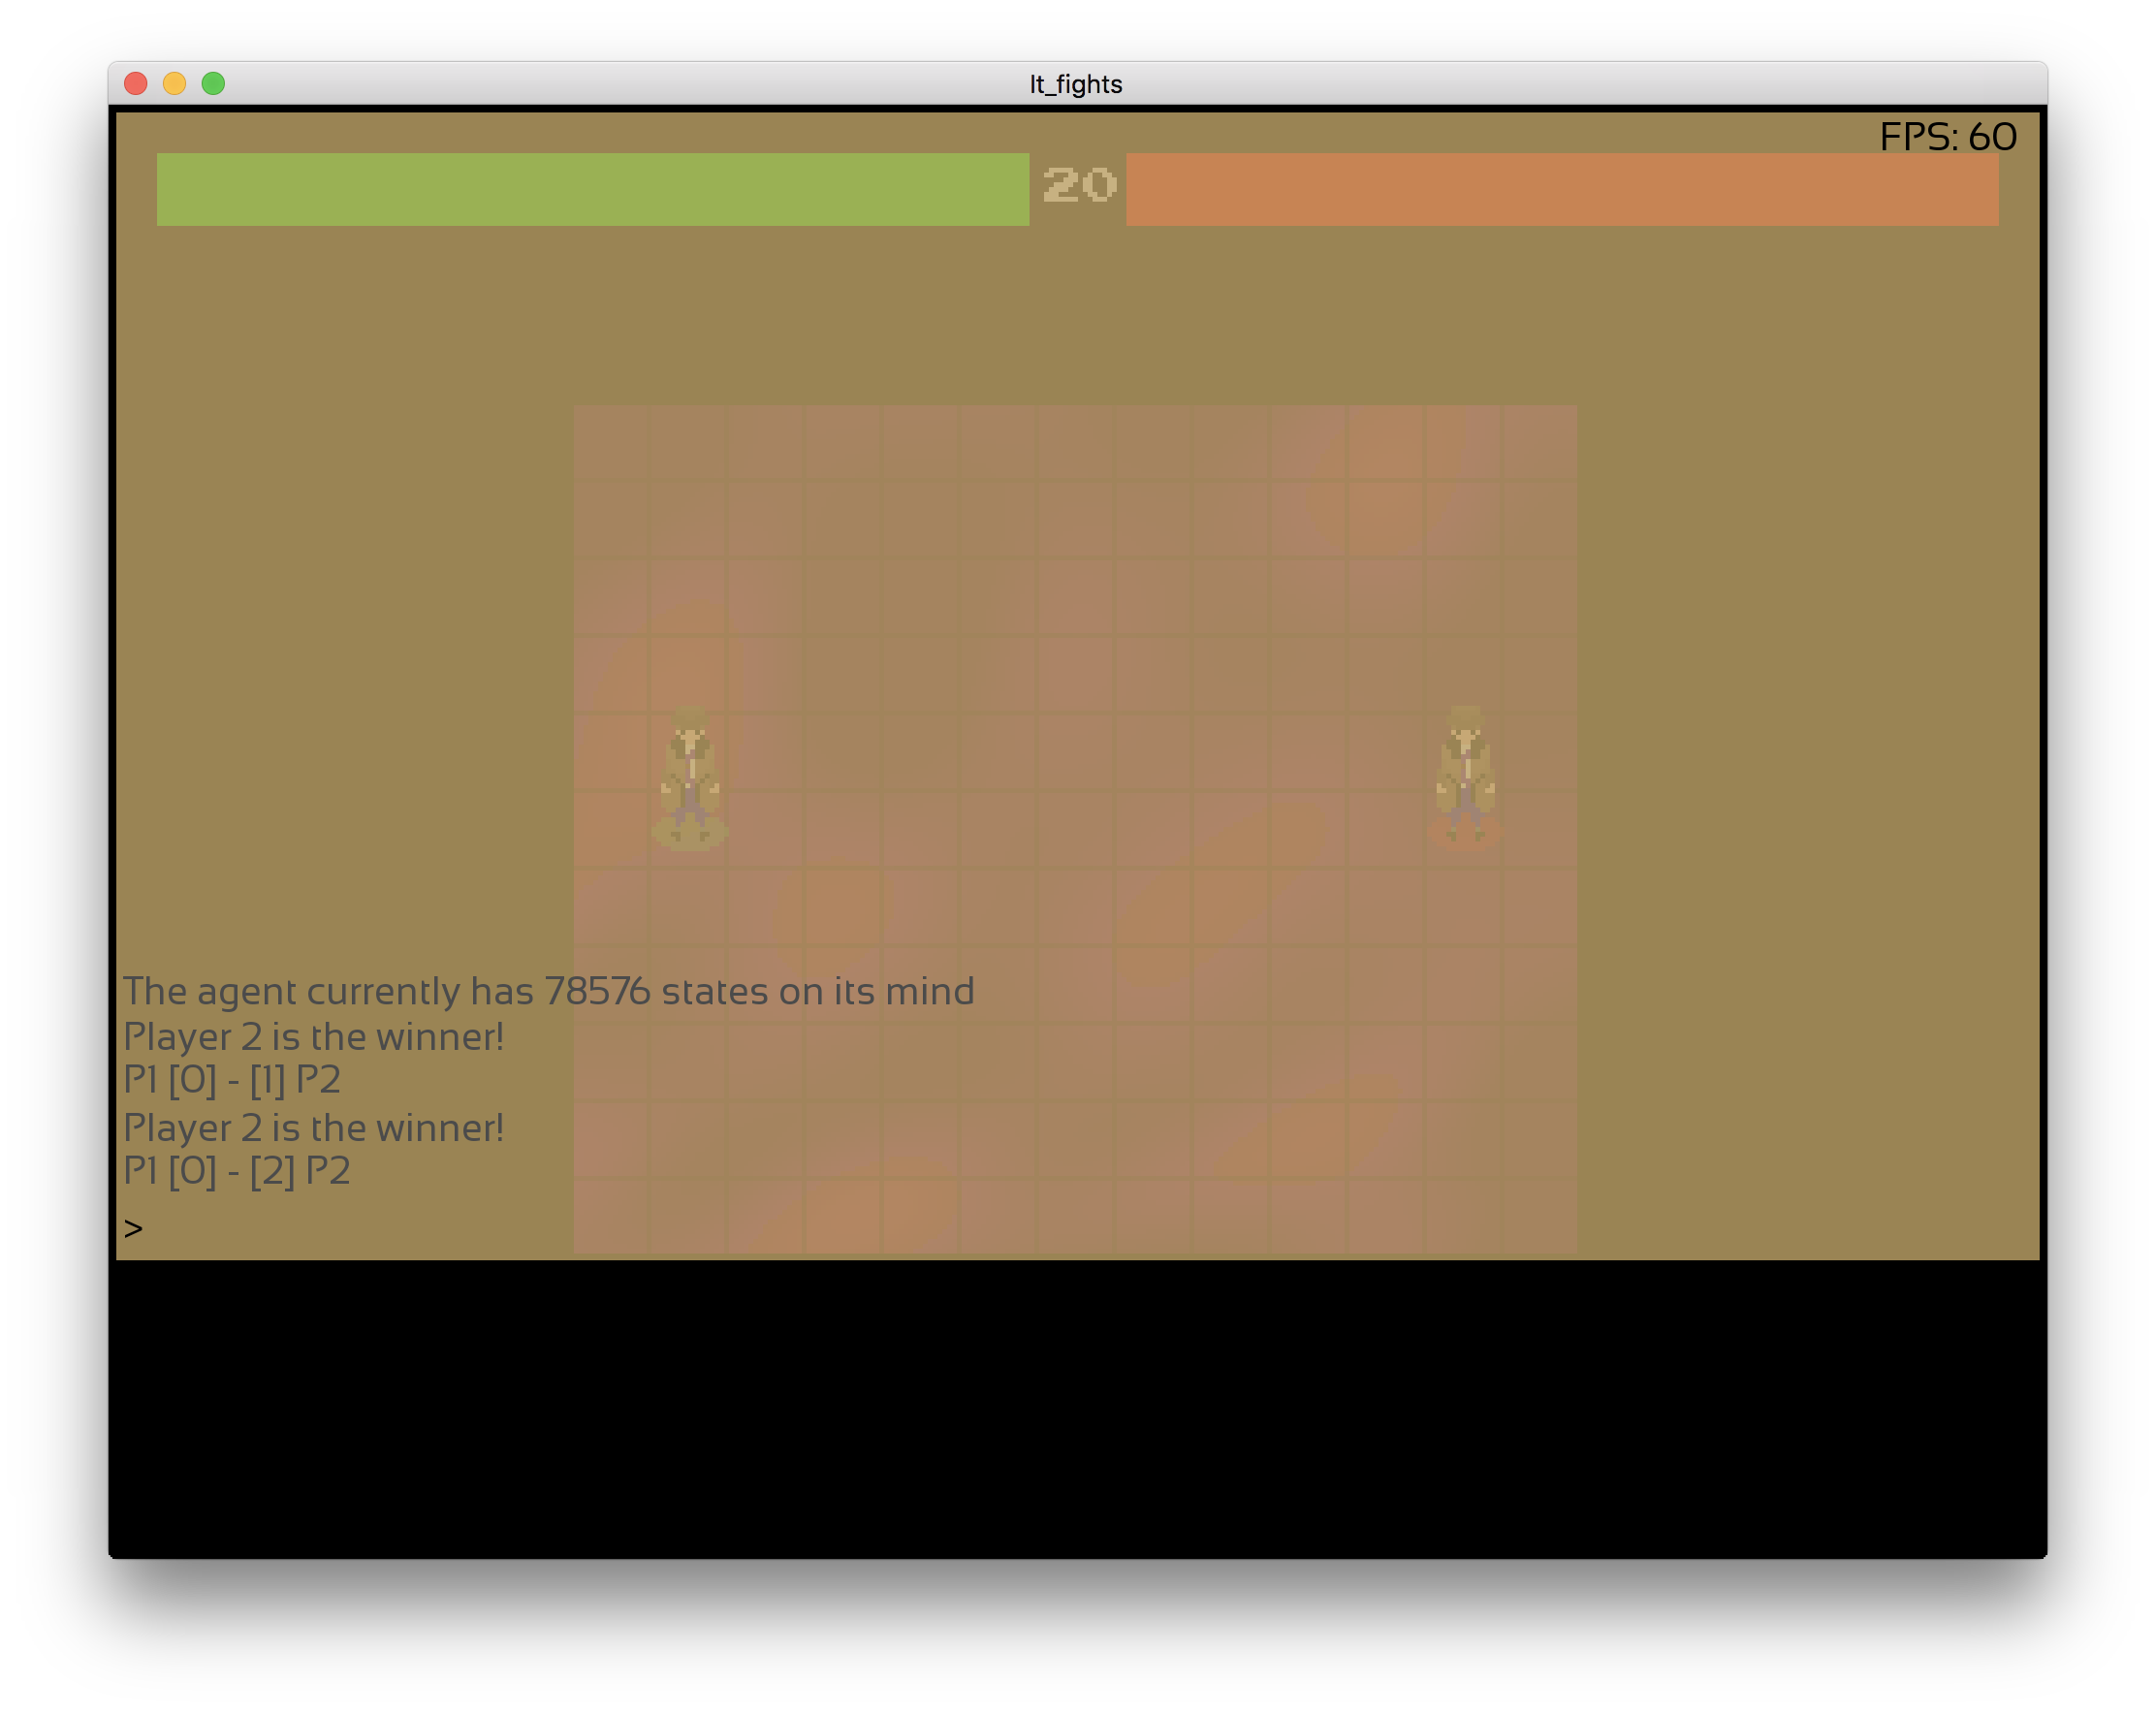
\includegraphics[width=17cm]{otros/manual/consola.png}}
	\caption{Consola abierta en la escena de combate}
	\label{uso:consola}
\end{figure}

Por último, se puede observar la consola abierta durante la escena de combate en la figura \ref{uso:consola}, la misma se puede abrir en cualquier momento del juego excepto cuando se están realizando las simulaciones sin \textit{renderizado} ya que no se muestra nada por pantalla para acelerar el proceso.

\bigskip

Con la consola abierta podemos ver los diferentes mensajes que se muestran en ella, en el caso de esta figura (\ref{uso:consola}) se puede ver el número de estados que había visitado el agente y las veces que uno de los personajes ha ganado al otro en esta ejecución.

\bigskip

Finalmente, se muestran los fotogramas por segundo o \textbf{\textit{FPS}} en la esquina superior derecha para ayudar a reconocer problemas de rendimiento si fuera necesario.


